\begin{enumerate}
\item
\begin{align}
\begin{split}
\myvec{5 & -4 }\vec{x}&=-8
\\
\myvec{7 & 6 }\vec{x}&=9
\end{split}
\end{align}
The above equations can be expressed as the matrix equation
\begin{align}
\myvec{5 & -4\\7 & 6} \vec{x} = \myvec{-8\\9}
\end{align}
%
The augmented matrix for the above equation is row reduced as follows
\begin{align}
\myvec{5 & -4 & -8\\7 & 6 & 9} 
\xleftrightarrow {R_1\leftarrow \ 7\frac{R_1}{5}}\myvec{7 & \frac{-28}{5} & \frac{-56}{5}\\7 & 6 & 9} 
\\
%\myvec{7 & \frac{-28}{5} &\frac{-56}{5} \\0 & \frac{58}{5} & \frac{101}{5}} 
\xleftrightarrow {R_2\leftarrow R_2 - R_1}\myvec{7 & \frac{-28}{5} &\frac{-56}{5} \\0 & \frac{58}{5} & \frac{101}{5}}
\\
%\myvec{5 & -4 & -8 \\0 & \frac{58}{5} & \frac{101}{5}} 
\xleftrightarrow {R_1\leftarrow 5\frac{R_1}{7}}\myvec{5 & -4 & -8 \\0 & \frac{58}{5} & \frac{101}{5}}
\\
%\myvec{5 & -4 & -8 \\0 & 58 & 101} 
\xleftrightarrow {R_2\leftarrow 5R_2}\myvec{5 & -4 & -8 \\0 & 58 & 101 }
\end{align}
%
$\because$ row reduction of the $2\times 3$ matrix
%
\begin{align}
\myvec{5 & -4 & -8\\7 & 6 & 9} \label{line/6/2.0.7}
\end{align}
%
results in a matrix with 2 nonzero rows, its rank is 2. 
%
Similarly, the rank of the matrix 
\begin{align}
\myvec{5 & -4 \\7 & 6 } \label{line/6/2.0.8}
\end{align}
%
is also 2.
%
\begin{align}
\because Rank \myvec{5 & -4\\7 & 6} &= Rank\myvec{5 & -4 & -8\\7 & 6 & 9} \nonumber\\
 &=dim \myvec{5 & -4\\7 & 6}\nonumber\\
 &=2
\end{align}

$\therefore$ the lines given in \eqref{line/6/1.0.1} intersect and are plotted in Fig. \ref{line/6/fig:INTERSECTING LINES.}.

\begin{figure}[ht!]
        \centering
        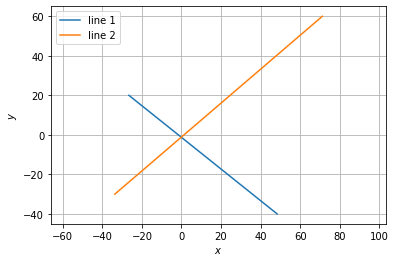
\includegraphics[width=\columnwidth]{solutions/su2021/2/6/FIGURES/INTERSECTING_LINES.png}
        \caption{INTERSECTING LINES.}
        \label{line/6/fig:INTERSECTING LINES.}
    \end{figure} 
    

\item
\begin{align}
\begin{split}
\myvec{9 & 3 }\vec{x}&=-12
\\
\myvec{18 & 6 }\vec{x}&=-24
\end{split}
\end{align}

The above equations can be expressed as the matrix equation
\begin{align}
\myvec{9 & 3\\18 & 6} \vec{x} = \myvec{-12\\-24}
\end{align}
%
The augmented matrix for the above equation is row reduced as follows
\begin{align}
\myvec{9 & 3 & -12\\18 & 6 & -24 } 
\xleftrightarrow {R_1\leftarrow \ 7\frac{R_1}{5}}\myvec{7 & \frac{-28}{5} & \frac{-56}{5}\\7 & 6 & 9} 
\\
%\myvec{18 & 6 & -24} \\18 & 6 & -24 
\xleftrightarrow {R_1\leftarrow \frac{18R_1}{9}}\myvec{18 & 6 & -24 \\18 & 6 & -24}
\\
%\myvec{18 & 6 & -24 \\0 & 0 & 0} 
\xleftrightarrow {R_2\leftarrow R_2-R_1}\myvec{18 & 6 & -24 \\0 & 0 & 0}
\end{align}
%
$\because$ row reduction of the $2\times 3$ matrix
%
\begin{align}
\myvec{9 & 3 & -12\\18 & 6 & -24}
\end{align}
%
results in a matrix with 1 nonzero rows, its rank is 1. 
%
Similarly, the rank of the matrix 
\begin{align}
\myvec{9 & 3 \\18 & 6 } 
\end{align}
%
is also 1.
%
\begin{align}
\because Rank \myvec{9 & 3\\18 & 6} &= Rank\myvec{9 & 3 & -12\\18 & 6 & -24}=1\nonumber\\
&< dim\myvec{9 & 3\\18 & 6}=2
\end{align}
%
$\therefore$ the lines \eqref{line/6/1.0.2} coincide and are plotted in Fig. \ref{line/6/fig:SAME LINES.}.
%
\begin{figure}[ht!]
    \centering
    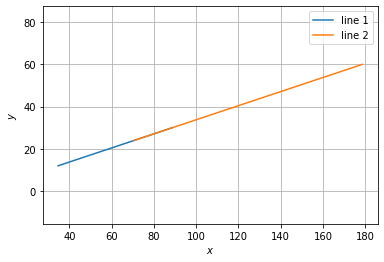
\includegraphics[width=\columnwidth]{solutions/su2021/2/6/FIGURES/SAME_LINES.png}
    \caption{SAME LINES}
    \label{line/6/fig:SAME LINES.}
\end{figure} 
%
\item
\begin{align}
\begin{split}
\myvec{6 & -3 }\vec{x}&=-10
\\
\myvec{2 & -1 }\vec{x}&=-9
\end{split}
\end{align}

The above equations can be expressed as the matrix equation
\begin{align}
\myvec{6 & -3\\2 & -1} \vec{x} = \myvec{-10\\-9}
\end{align}
%
The augmented matrix for the above equation is row reduced as follows
\begin{align}
\myvec{6 & -3 & -10\\2 & -1 & -9 } 
\xleftrightarrow {R_1\leftarrow \ \frac{2R_1}{6}}\myvec{2 & -1 & \frac{-10}{3}\\2 & -1 & -9} 
\\
%\myvec{2 & -1 & \frac{-10}{3} \\0 & 0 & \frac{-17}{3} 
\xleftrightarrow {R_2\leftarrow R_2-R_1}\myvec{2 & -1 & \frac{-10}{3} \\0 & 0 & \frac{-17}{3} }
\\
%\myvec{6 & -3 & -10 \\0 & 0 & \frac{-17}{3}} 
\xleftrightarrow {R_1\leftarrow 3R_1}\myvec{6 & -3 & -10 \\0 & 0 & \frac{-17}{3}} 
\end{align}
%
$\because$ row reduction of the $2\times 3$ matrix
%
\begin{align}
\myvec{6 & -3 & -10\\2 & -1 & -9}
\end{align}
%
results in a matrix with 2 nonzero rows, its rank is 2. 
%
Similarly, the rank of the matrix 
\begin{align}
\myvec{6 & -3 \\2 & -1 } 
\end{align}
%
is 1.
%
\begin{align}
\because Rank \myvec{6 & -3 \\2 & -1 } \ne Rank \myvec{6 & -3 & -10\\2 & -1 & -9}
\end{align}
$\therefore$ the lines in  \eqref{line/6/1.0.3} are parallel and plotted in Fig.     \ref{line/6/fig: PARALLEL lines.}.
%
\begin{figure}[ht]
    \centering
   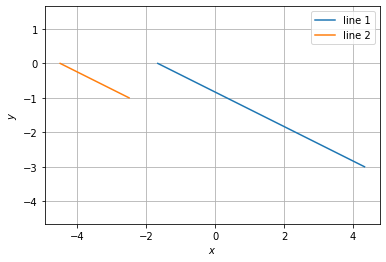
\includegraphics[width=\columnwidth]{solutions/su2021/2/6/FIGURES/PARALLEL_LINES.png}
    \caption{Parallel lines}
    \label{line/6/fig: PARALLEL lines.}
\end{figure}    
\end{enumerate}
